\documentclass{article}
\usepackage[utf8]{inputenc}
\usepackage[letterpaper, total={6in, 9in}]{geometry}
\usepackage{amsmath}
\usepackage{natbib}
\usepackage{wrapfig}
\usepackage{graphicx}

\title{Geometry 2 - Circles}
\author{TSS Math Club}
\date{Oct 2022}

\graphicspath{ {./geo2/} }

\begin{document}
\large

\maketitle

\section{Basic property of Circles}
\subsection{Definition of Circles}
\subsection{Terms to describe geometric object related to circles}
\begin{wrapfigure}{R}{0.4\textwidth} %this figure will be at the right
    \centering
    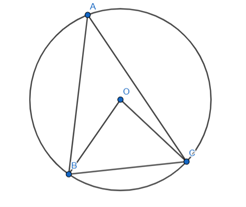
\includegraphics[width=0.4\textwidth]{Picture1.png}
\end{wrapfigure}
Center: \\ \\
Radius: \\ \\
Arc: \\ \\
Chord: \\ \\
Central angle: \\ \\
Inscribed angle: \\ \\


\subsection{Central angle is twice any inscribed angle}
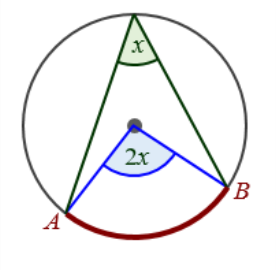
\includegraphics{Picture2.png}

\pagebreak

\subsection{Inscribed angles subtended by the same arc are equal}

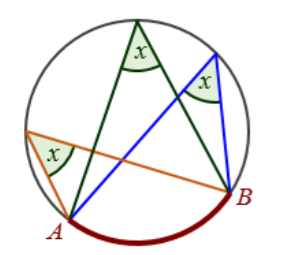
\includegraphics{Picture3.png}

\vspace{40px}

\subsection{Angle subtended by a diameter is \(90^{\circ}\)}

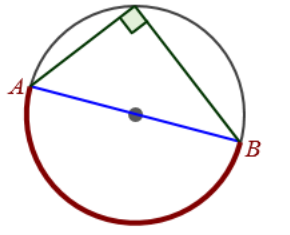
\includegraphics{Picture4.png}

\pagebreak

\subsection{Perpendicular chord theorem}

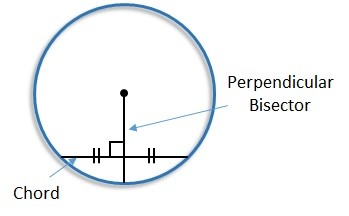
\includegraphics{Picture5.jpg}

\vspace{50px}

\subsection{Tangent to a circle}

\subsubsection{Definition:}
\vspace{20px}

\subsubsection{The radius from the center of the circle to the point of tangency is perpendicular to the tangent line}

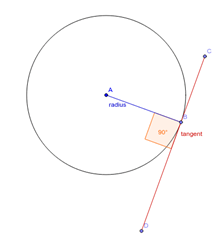
\includegraphics{Picture6.png}

\pagebreak

\subsubsection{The length of tangents from a point to a circle are equal}

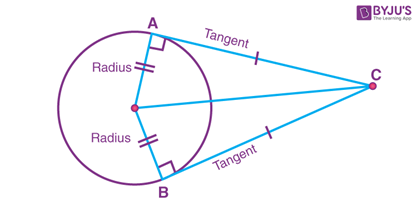
\includegraphics{Picture7.png}

\vspace{50px}

\subsubsection{Tangent-Chord Theorem: the angle formed between a chord and a tangent line to a circle is equal to the inscribed angle on the other side of the chord}

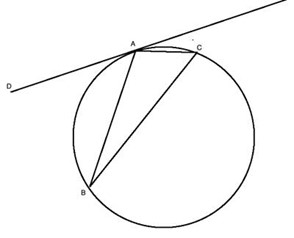
\includegraphics{Picture8.jpg}

\pagebreak

\section{Cyclic Quadrilateral (Four points cyclic)}

\subsection{Definition}

\vspace{20px}

\subsection{Opposite angles are added up to \(180^{\circ}\)}

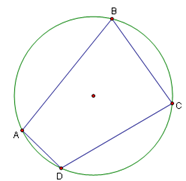
\includegraphics[scale=.8]{Picture9.png}

\subsection{How to prove four points cyclic}

\subsubsection{Prove these four points lies equally distance to another point — the center of the circle}

\subsubsection{Two equal angles subtend a segment (chord in the circle)}

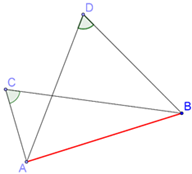
\includegraphics{Picture10.png}

\subsubsection{Opposite angles are added up to \(180^{\circ}\)}

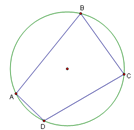
\includegraphics{Picture11.png}

\pagebreak

\section{Similar triangles involving a circle}

\subsection{Identify as many similar triangles as possible}

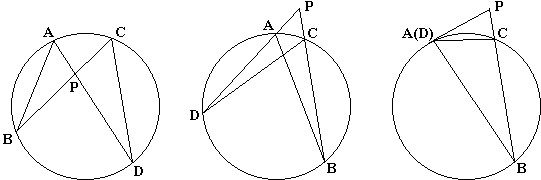
\includegraphics[scale=.75]{Picture12.jpg}

\vspace{100px}

\subsection{Power of a point}

\subsubsection{Definition:}

\vspace{20px}

\subsubsection{Power of point is fixed regardless the choice of chord}

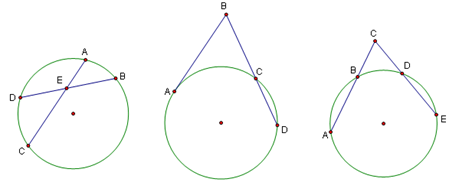
\includegraphics[scale=1.2]{Picture13.png}

\pagebreak

\subsubsection{Power of a point formula}

\[PoP = {PO}^2+r^2\]

\begin{center}
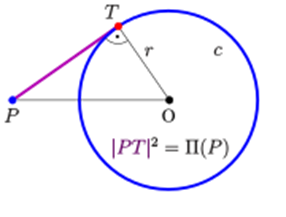
\includegraphics{Picture14.png}
\end{center}

\vspace{60px}

\subsection{Homothety involving circles}

\subsubsection{Homothety of a circle is a circle}

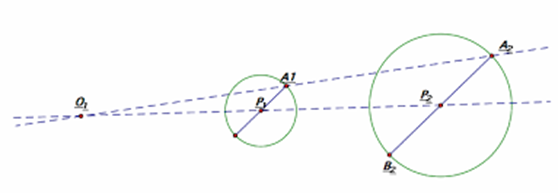
\includegraphics{Picture15.png}

\subsubsection{Ratios in the homothety}

\pagebreak

\section{Problems}

\subsection{Problem}
Given AD AE are the internal, external angle bisector of angle A,
 such that D,E are the intersection of the angle bisectors with the circumcircle. 
 Prove DE is a diameter of the circle.

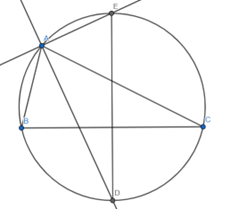
\includegraphics{Picture16.png}

\vspace{50px}

\subsection{Problem}
Given Circle C1, C2 intersect at A, B, CD is the common tangent to both circles, 
E is the intersection of AB and CD. Prove E is the midpoint of CD.

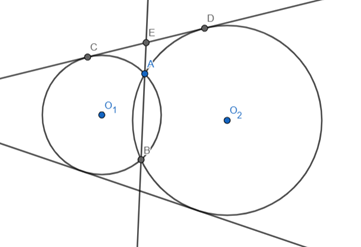
\includegraphics{Picture17.png}

\pagebreak

\subsection{Theorem}
In a triangle abc=4RS

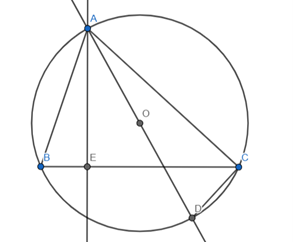
\includegraphics{Picture18.png}

\pagebreak

\subsection{Problem}

Given AE is the external angle bisector of angle A, 
AE intersects BC at G, 
the tangent at A intersects BC at F. 
Prove AFG is an isosceles triangle.

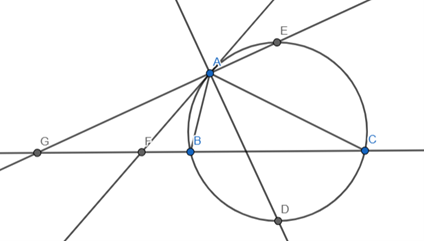
\includegraphics{Picture19.png}

\pagebreak

\subsection{Ptolemy's theorem}

If a quadrilateral is inscribable in a circle then the product of the lengths of its diagonals is equal to the sum of the products of the lengths of the pairs of opposite sides.
\\Or ab+cd=xy where a,b,c,d are the sides of the quadrilateral and x,y are the diagonals.

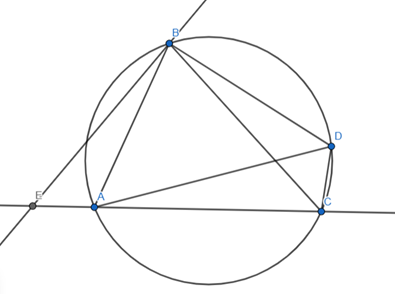
\includegraphics{Picture20.png}

\pagebreak

\subsection{Problem}
In \(\triangle\)ABC, point D is inside of ABC such that \(\angle DAC = \angle DCA=30^{\circ} \) and \(\angle DBA=60^{\circ}\). E is the midpoint on BC and F is a trisect point on AC such that \(CF = \frac{CA}{3} \). Prove DE \(\perp\) EF.

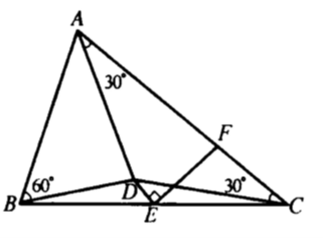
\includegraphics{Picture21.png}

\end{document}
